\section{Inverse Functions}

\subsection{Definition}

Let $f$ be some function of a variable $x$, that is $f=f(x)$.  The {\bf inverse function} of $f$, is some function $g$ such that $g(f(x))=x$.  The inverse of a function acts to "undo" whatever a function does.\\

To find the inverse of a function $f(x)$, write out the full equation, and substitute every instance of $x$ with $f^{-1}(x)$, and every instance of $f(x)$ with $x$.  You should be left with an equation in terms of $f^{-1}(x)$ and $x$.  Work to isolate $f^{-1}(x)$, and the result will be an equation for the inverse of $f(x)$.  For example,\\

\tab$f(x) = x^2 + 1$\\

\tab$\implies x = (f^{-1}(x))^2 + 1$\\

\tab$\implies x - 1 = (f^{-1}(x))^2$\\

\tab$\implies f^{-1}(x) = \sqrt{(x - 1)}$\\

Keep in mind it is not always possible to find the inverse of a function.  While the inverse of a function is always a {\bf relation}, it is not always a function, in which case it would be impossible to isolate $f^-1(x)$.\\

To find the inverse of a function graphically, take a graph of the function, and switch the x and y axes.  The inverse of a function maps its output back to its input, thus the x and y coordinates of every point in the function should be switched.\\

\subsection{Inverse Sinse}

As mentioned before, the sine is a function that maps an angle to a ratio.\\

\tab$sin(\theta) = \frac{y}{r}$\\

The inverse sine, also called the {\bf arc-sine}, is the function where\\

\tab$arcsin(\frac{y}{r}) = \theta$\\

or a function that takes in a ratio, and outputs an angle.\\

\begin{figure}[htb!]
\center
\caption{Graph of arc-sine.}
\label{fig:graph of arc-sine}
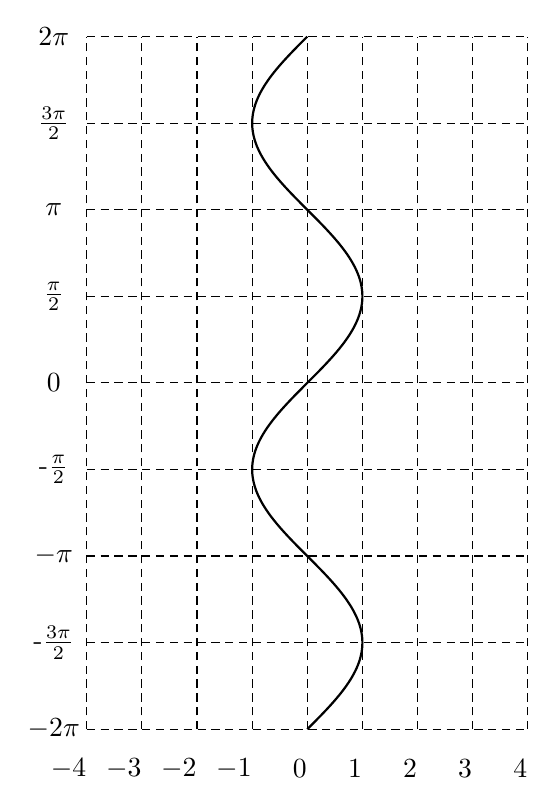
\begin{tikzpicture}[inner sep=0pt,minimum size=0mm, scale = 0.7]

\node at (-4.6,3.1415) {$\pi$};
\node at (-4.6,3/2*3.1415) {$\frac{3\pi}{2}$};
\node at (-4.6,2*3.1415) {$2\pi$};
\node at (-4.6,1/2*3.1415) {$\frac{\pi}{2}$};
\node at (-4.6,0) {$0$};
\node at (-4.6,1/2*-3.1415) {-$\frac{\pi}{2}$};
\node at (-4.6,-3.1415) {$-\pi$};
\node at (-4.6,3/2*-3.1415) {-$\frac{3\pi}{2}$};
\node at (-4.6,2*-3.1415) {$-2\pi$};

\node[left] at (4, -7) {$4$};
\node[left] at (3, -7) {$3$};
\node[left] at (2, -7) {$2$};
\node[left] at (1, -7) {$1$};
\node[left] at (0, -7) {$0$};
\node[left] at (-1, -7) {$-1$};
\node[left] at (-2, -7) {$-2$};
\node[left] at (-3, -7) {$-3$};
\node[left] at (-4, -7) {$-4$};

\draw[ystep=3.1415/2, densely dashed] (-4,-2*3.1415) grid (4,2*3.1415);
\AXES{0}{0}{4}{2*3.1415}
\draw[thick, variable = \t, domain=2*-3.1415:2*3.1415,samples=250] plot ({sin(180*\t/3.1415)},{\t});

\end{tikzpicture}
\end{figure}

Note the difference in domain and range:  The sine is a function that takes in an angle, and maps it to a ratio, whereas the arcsine takes in a ratio and maps it to an angle.\\

There are also an inverse cosine, the {\bf arc-cosine}, and and inverse tangent, the {\bf arc-tangent}.\\

\tab$arccos(\frac{x}{r}) = \theta$\\

\tab$arctan(\frac{y}{x}) = \theta$\\

\begin{figure}[htb!]
\center
\caption{Graph of arc-cosine.}
\label{fig:graph of arc-cosine}
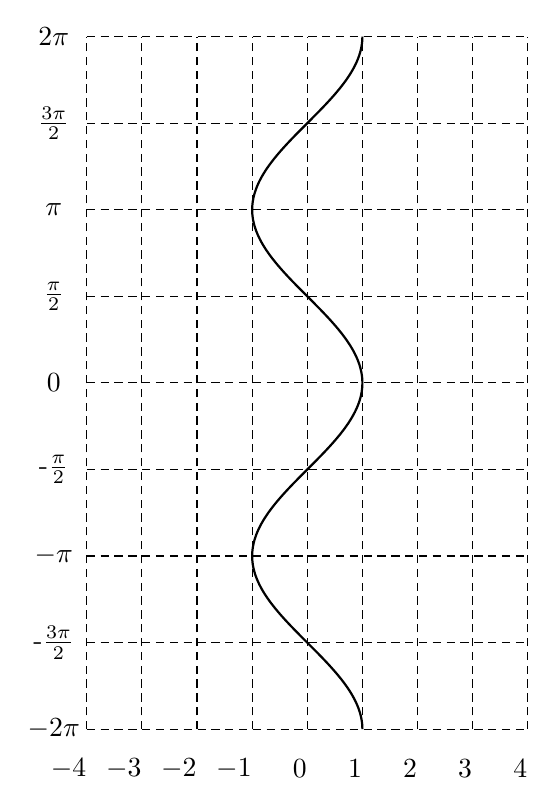
\begin{tikzpicture}[inner sep=0pt,minimum size=0mm, scale = 0.7]

\node at (-4.6,3.1415) {$\pi$};
\node at (-4.6,3/2*3.1415) {$\frac{3\pi}{2}$};
\node at (-4.6,2*3.1415) {$2\pi$};
\node at (-4.6,1/2*3.1415) {$\frac{\pi}{2}$};
\node at (-4.6,0) {$0$};
\node at (-4.6,1/2*-3.1415) {-$\frac{\pi}{2}$};
\node at (-4.6,-3.1415) {$-\pi$};
\node at (-4.6,3/2*-3.1415) {-$\frac{3\pi}{2}$};
\node at (-4.6,2*-3.1415) {$-2\pi$};

\node[left] at (4, -7) {$4$};
\node[left] at (3, -7) {$3$};
\node[left] at (2, -7) {$2$};
\node[left] at (1, -7) {$1$};
\node[left] at (0, -7) {$0$};
\node[left] at (-1, -7) {$-1$};
\node[left] at (-2, -7) {$-2$};
\node[left] at (-3, -7) {$-3$};
\node[left] at (-4, -7) {$-4$};

\draw[ystep=3.1415/2, densely dashed] (-4,-2*3.1415) grid (4,2*3.1415);
\AXES{0}{0}{4}{2*3.1415}
\draw[thick, variable = \t, domain=2*-3.1415:2*3.1415,samples=250] plot ({cos(180*\t/3.1415)},{\t});

\end{tikzpicture}
\end{figure}

\begin{figure}[htb!]
\center
\caption{Graph of arc-tangent.}
\label{fig:graph of arc-tan}
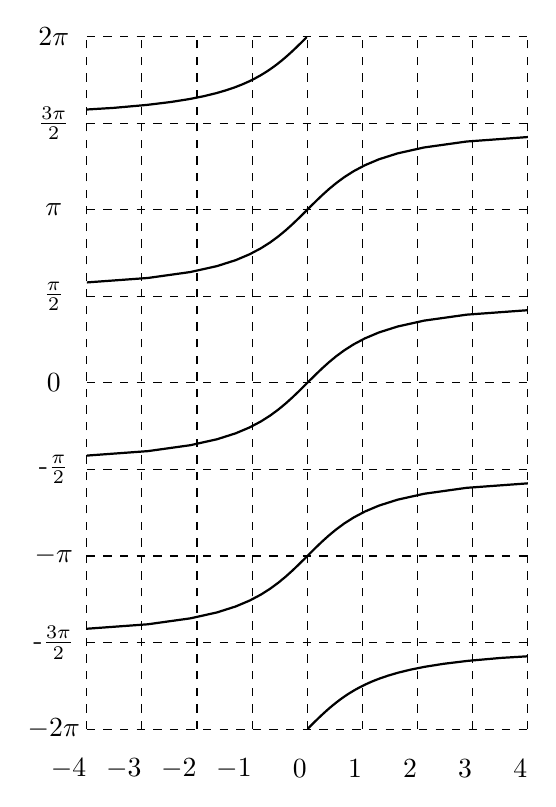
\begin{tikzpicture}[inner sep=0pt,minimum size=0mm, scale = 0.7]

\node at (-4.6, 3.1415) {$\pi$};
\node at (-4.6, 3/2*3.1415) {$\frac{3\pi}{2}$};
\node at (-4.6, 2*3.1415) {$2\pi$};
\node at (-4.6, 1/2*3.1415) {$\frac{\pi}{2}$};
\node at (-4.6, 0) {$0$};
\node at (-4.6, 1/2*-3.1415) {-$\frac{\pi}{2}$};
\node at (-4.6, -3.1415) {$-\pi$};
\node at (-4.6, 3/2*-3.1415) {-$\frac{3\pi}{2}$};
\node at (-4.6, 2*-3.1415) {$-2\pi$};

\node[left] at (4, -7) {$4$};
\node[left] at (3, -7) {$3$};
\node[left] at (2, -7) {$2$};
\node[left] at (1, -7) {$1$};
\node[left] at (0, -7) {$0$};
\node[left] at (-1, -7) {$-1$};
\node[left] at (-2, -7) {$-2$};
\node[left] at (-3, -7) {$-3$};
\node[left] at (-4, -7) {$-4$};

\draw[ystep=3.1415/2, dashed] (-4,-2*3.1415) grid (4,2*3.1415);
\AXES{0}{0}{4}{2*3.1415}

\begin{scope}
    \clip(-4, 2*-3.1415) rectangle (4, 2*3.1415);

\draw[thick,
 variable = \t, 
 domain=4/2*-3.1415+0.01:3/2*-3.1415-0.01,
 samples=30] 
plot ({tan(180*\t/3.1415)}, {\t});


\draw[thick,
 variable = \t, 
 domain=3/2*-3.1415+0.01:1/2*-3.1415-0.01,
 samples=30] 
plot ({tan(180*\t/3.1415)}, {\t});

\draw[thick,
 variable = \t, 
 domain=1/2*-3.1415+0.01:1/2*3.1415-0.01,
 samples=30] 
plot ({tan(180*\t/3.1415)}, {\t});

\draw[thick,
 variable = \t, 
 domain=1/2*3.1415+0.01:3/2*3.1415-0.01,
 samples=30] 
plot ({tan(180*\t/3.1415)}, {\t});

\draw[thick,
 variable = \t, 
 domain=3/2*3.1415+0.01:4/2*3.1415-0.01,
 samples=30] 
plot ({tan(180*\t/3.1415)}, {\t});

\end{scope}

\end{tikzpicture}
\end{figure}

\subsection{Principal Angles}

However, due to the periodicity of the trigonometric functions, the inverse trigonometric functions are not strictly functions.  Remember that\\

\tab$sin(\theta) = sin(\theta \pm 2\pi n), \ \ n=0,1,2,...$\\

From this we can say that\\

\tab$sin(\theta \pm 2\pi n) = \frac{y}{r}$\\

Taking the inverse of both sides leaves us with\\

\tab$arcsin(sin(\theta + 2\pi n)) = arcsin(\frac{y}{r})$\\

\tab$\theta + 2\pi n = arcsin(\frac{y}{r})$\\

The arcsine is a {\bf relation}, but is not strictly a {\bf function}, since for every input value $\frac{y}{r}$, there is an infinite set of possible output values $\theta + 2\pi n$.  The typical approach to handling this shortcoming is to constrain the inverse trig functions to a certain range, called the {\bf principal-value range}.  By doing this, we create equivalent inverses that are functions.\\

\begin{figure}[htb!]
\center
\caption{Arc-sine constrained to its principal-value range.}
\label{fig:principal value arc sine}
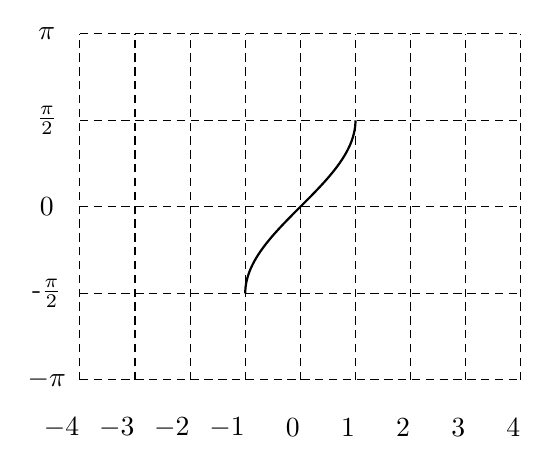
\begin{tikzpicture}[inner sep=0pt,minimum size=0mm, scale = 0.7]

\node at (-4.6,3.1415) {$\pi$};
\node at (-4.6,1/2*3.1415) {$\frac{\pi}{2}$};
\node at (-4.6,0) {$0$};
\node at (-4.6,1/2*-3.1415) {-$\frac{\pi}{2}$};
\node at (-4.6,-3.1415) {$-\pi$};

\node[left] at (4, -4) {$4$};
\node[left] at (3, -4) {$3$};
\node[left] at (2, -4) {$2$};
\node[left] at (1, -4) {$1$};
\node[left] at (0, -4) {$0$};
\node[left] at (-1, -4) {$-1$};
\node[left] at (-2, -4) {$-2$};
\node[left] at (-3, -4) {$-3$};
\node[left] at (-4, -4) {$-4$};

\draw[ystep=3.1415/2, densely dashed] (-4,-1*3.1415) grid (4,1*3.1415);
\AXES{0}{0}{4}{1*3.1415}
\draw[thick, variable = \t, domain=1/2*-3.1415:1/2*3.1415,samples=250] plot ({sin(180*\t/3.1415)},{\t});

\end{tikzpicture}
\end{figure}

\begin{figure}[htb!]
\center
\caption{Arc-cosine constrained to its principal-value range.}
\label{fig:principal value arc-cosine }
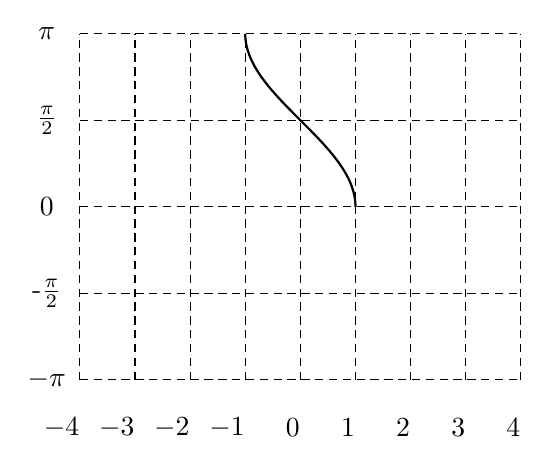
\begin{tikzpicture}[inner sep=0pt,minimum size=0mm, scale = 0.7]

\node at (-4.6,3.1415) {$\pi$};
\node at (-4.6,1/2*3.1415) {$\frac{\pi}{2}$};
\node at (-4.6,0) {$0$};
\node at (-4.6,1/2*-3.1415) {-$\frac{\pi}{2}$};
\node at (-4.6,-3.1415) {$-\pi$};

\node[left] at (4, -4) {$4$};
\node[left] at (3, -4) {$3$};
\node[left] at (2, -4) {$2$};
\node[left] at (1, -4) {$1$};
\node[left] at (0, -4) {$0$};
\node[left] at (-1, -4) {$-1$};
\node[left] at (-2, -4) {$-2$};
\node[left] at (-3, -4) {$-3$};
\node[left] at (-4, -4) {$-4$};

\draw[ystep=3.1415/2, densely dashed] (-4,-1*3.1415) grid (4,1*3.1415);
\AXES{0}{0}{4}{1*3.1415}
\draw[thick, variable = \t, domain=0:3.1415,samples=250] plot ({cos(180*\t/3.1415)},{\t});

\end{tikzpicture}
\end{figure}


\begin{figure}[htb!]
\center
\caption{Arc-tangent contrained to its principal-value range.}
\label{fig:principal value arc-tan}
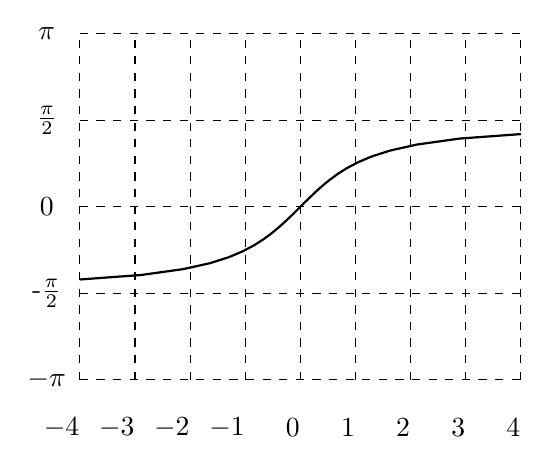
\begin{tikzpicture}[inner sep=0pt,minimum size=0mm, scale = 0.7]

\node at (-4.6, 3.1415) {$\pi$};
\node at (-4.6, 1/2*3.1415) {$\frac{\pi}{2}$};
\node at (-4.6, 0) {$0$};
\node at (-4.6, 1/2*-3.1415) {-$\frac{\pi}{2}$};
\node at (-4.6, -3.1415) {$-\pi$};

\node[left] at (4, -4) {$4$};
\node[left] at (3, -4) {$3$};
\node[left] at (2, -4) {$2$};
\node[left] at (1, -4) {$1$};
\node[left] at (0, -4) {$0$};
\node[left] at (-1, -4) {$-1$};
\node[left] at (-2, -4) {$-2$};
\node[left] at (-3, -4) {$-3$};
\node[left] at (-4, -4) {$-4$};

\draw[ystep=3.1415/2, dashed] (-4,-3.1415) grid (4,3.1415);
\AXES{0}{0}{4}{3.1415}

\begin{scope}
    \clip(-4, -3.1415) rectangle (4, 3.1415);

\draw[thick,
 variable = \t, 
 domain=1/2*-3.1415+0.01:1/2*3.1415-0.01,
 samples=30] 
plot ({tan(180*\t/3.1415)}, {\t});

\end{scope}

\end{tikzpicture}
\end{figure}

The following table lists the principal-value range for the inverse trigonometric functions.\\

\begin{figure}[htb!]
\caption{Principal-value range for inverse trigonometric functions.}
\label{fig:principal_value_range}
\begin{center}
\begin{tabular}{ | c | c | }
\hline 
function & principal-value range\\
\hline 
$arcsin(\theta)$ & $-\pitwo \leq \theta \leq \pitwo$ \\
\hline 
$arccos(\theta)$ & $0 \leq \theta \leq \pi$ \\
\hline 
$arctan(\theta)$ & $-\pitwo < \theta < \pitwo$ \\
\hline 
$arcsec(\theta)$ & $0 \leq \theta \leq \pi, \theta \neq \pitwo$ \\
\hline 
$arccsc(\theta)$ & $-\pitwo \leq \theta \leq \pitwo, \theta \neq 0$ \\
\hline 
$arccot(\theta)$ & $0 < \theta < \pi$ \\
\hline
\end{tabular}
\end{center}
\end{figure}

\clearpage
\subsection{Review}

\begin{enumerate}

\item{What is the definition of the inverse of a function?}\\

\item{Write the inverse of each of the following functions:}\\

\tab a) $f(x) = x + 1$\\

\tab b) $f(x) = x^2$\\

\tab c) $f(x) = \frac{1}{x}$\\

\tab d) $f(x) = sin(x)$\\

\tab e) $f(x) = 1$\\

\item{What is the difference between a relation and a function?}\\

\item{Why do inverse trig. functions have a principal-value range?}\\

\item{Draw and label a graph of the arc-sine, arc-cosine, and arc-tangent, without referring back to the text.}\\

\end{enumerate}
